\documentclass[12pt]{article}

\usepackage{sbc-template}

\usepackage{graphicx,url}

\usepackage[brazil]{babel}
%\usepackage[latin1]{inputenc}
\usepackage[utf8]{inputenc}
% UTF-8 encoding is recommended by ShareLaTex

\usepackage{hyperref}

\usepackage{pdftexcmds}
\usepackage{minted}

\setminted{frame=lines}

\sloppy

\title{Bancos de Dados Geográficos}

\author{Fuad Saud\inst{1}, Luiz Felipe Cunha\inst{1}, Ramon Saraiva\inst{1}}

\address{Universidade do Vale do Rio dos Sinos
  \email{\{fuadfsaud,felipe.silvacunha\}@gmail.com}
}

\begin{document}

\maketitle

\begin{abstract}
  This paper gives an overview of the state of the art GIS-aware database
  management systems and introduces the PostGIS extension to the popular
  open source RDBMS PostgreSQL by means of examples.
\end{abstract}

\begin{resumo}
  Este artigo apresenta um apanhado do estado da arte com relação a sistemas de
  gerenciamento de bancos de dados com suporte a processamento geográfico e
  introduz o PostGIS, uma extensão do popular SGBDR PostgreSQL.
\end{resumo}


\section{Bancos de Dados Geográficos}

Por muito tempo, desde os primeiros dias dos sistemas de informação
geográficas, dados espaciais foram e ainda são armazenados em
\textit{shapefiles} - arquivos onde os dados são estruturados de forma plana
(não indexada) e que não oferecem nenhum tipo de acesso padronizado.

Utilizar um banco de dados relacional para o armazenamento e mediação de acesso
a dados geográficos oferece um leque de vantagens sobre estratégias de
armazenamento. Entre elas estão o uso do SQL como interface padrão para
interação com o banco de dados, o que permite tanto descrever computações e
relacionamentos complicados entre os dados de maneira simplificada como
combinar essas computações com outras computações relacionais triviais, levando
em conta todas as ferramentas existentes para trabalhar com bancos de dados
relacionais; acesso concorrente controlado de forma a evitar possíveis
corrupções na estrutura de armazenamento.

Algumas das tecnologias atuais de armazenamento e processamento de dados
geográficos são listadas a seguir:

\begin{description}
\item[PostGIS:] extensão para o SGBDR PostgreSQL que adiciona funcionalidades
  de armazenamento, busca e indexação geoespacial;
\item[MongoDB:]
\end{description}

\section{PostGIS} \label{sec:firstpage}

Como mencionado na seção anterior, o \href{http://postgis.net}{PostGIS} é uma
extensão que adiciona a capacidade de trabalhar com dados geográficos ao SGBDR
PostgreSQL. A primeira versão do projeto foi publicada em 2001 pela
\href{http://refractions.net}{Refractions Research} projeto de código aberto
foi publicada em 2001 sob a GNU General Public License, permitindo a aberta
distribuição do código-fonte e uso do programa.

A partir desta versão inicial, algumas funções foram padronizadas pelo Open
Geospatial Consortium, formando a especificação SFSQL ("Simple Features for
SQL"), que posteriormente passou a ser desenvolvida de maneira independente ao
PostGIS.

\subsection{Configuração}

A instalação da extensão é deveras fácil e pode ser feita em diferentes
plataformas de várias maneiras, como descrito na
\href{http://postgis.net/install}{Apágina de instalação do site oficial}.

Uma vez instalada, a extensão pode ser habilitada em uma base de dados por meio
do seguinte comando:

\begin{minted}{sql}
  CREATE EXTENSION postgis;
\end{minted}

Dados geográficos podem ser inseridos de várias modos. Uma maneira conveniente
é importar um shapefile inteiro para a base de dados, tarefa que pode ser
realizada com a ajuda da ferramenta \texttt{shp2pgsql}. Ela transforma um
shapefile em um script SQL que pode ser rodado diretamente na base de dados com
o PostGIS habilitado da seguinte forma:

\begin{minted}{shell}
  shp2pgsql /path/to/shapefile.shp > output.sql
  pgsql postgis_enabled_database < output.sql
\end{minted}

\section{Indexação}

Section titles must be in boldface, 13pt, flush left. There should be an extra
12 pt of space before each title. Section numbering is optional. The first
paragraph of each section should not be indented, while the first lines of
subsequent paragraphs should be indented by 1.27 cm.
R-tree, Quadtree, grid-based indexes.

\subsection{Subsections}

The subsection titles must be in boldface, 12pt, flush left.

\section{Figures and Captions}\label{sec:figs}


Figure and table captions should be centered if less than one line
(Figure~\ref{fig:exampleFig1}), otherwise justified and indented by 0.8cm on
both margins, as shown in Figure~\ref{fig:exampleFig2}. The caption font must
be Helvetica, 10 point, boldface, with 6 points of space before and after each
caption.

\begin{figure}[ht]
  \centering
  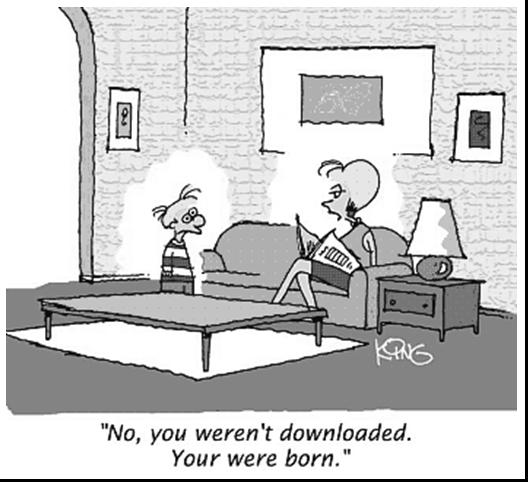
\includegraphics[width=.5\textwidth]{fig1.jpg}
  \caption{A typical figure}
  \label{fig:exampleFig1}
\end{figure}

\begin{figure}[ht]
  \centering
  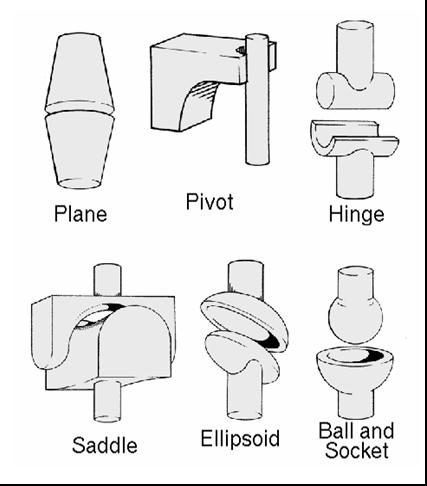
\includegraphics[width=.3\textwidth]{fig2.jpg}
  \caption{This figure is an example of a figure caption taking more than one
  line and justified considering margins mentioned in Section~\ref{sec:figs}.}
  \label{fig:exampleFig2}
\end{figure}

In tables, try to avoid the use of colored or shaded backgrounds, and avoid
thick, doubled, or unnecessary framing lines. When reporting empirical data,
do not use more decimal digits than warranted by their precision and
reproducibility. Table caption must be placed before the table (see Table 1)
and the font used must also be Helvetica, 10 point, boldface, with 6 points of
space before and after each caption.

\begin{table}[ht]
  \centering
  \caption{Variables to be considered on the evaluation of interaction
  techniques}
  \label{tab:exTable1}
  \smallskip
  \begin{tabular}{|l|c|c|}
    \hline
    & Value 1 & Value 2\\[0.5ex]
    \hline
    &&\\[-2ex]
    Case 1 & 1.0 $\pm$ 0.1 & 1.75$\times$10$^{-5}$ $\pm$ 5$\times$10$^{-7}$\\[0.5ex]
    \hline
    &&\\[-2ex]
    Case 2 & 0.003(1) & 100.0\\[0.5ex]
    \hline
  \end{tabular}
\end{table}

\section{Images}

All images and illustrations should be in black-and-white, or gray tones,
excepting for the papers that will be electronically available (on CD-ROMs,
internet, etc.). The image resolution on paper should be about 600 dpi for
black-and-white images, and 150-300 dpi for grayscale images.  Do not include
images with excessive resolution, as they may take hours to print, without any
visible difference in the result.

\section{References}

Bibliographic references must be unambiguous and uniform.  We recommend giving
the author names references in brackets, e.g. \cite{knuth:84},
\cite{boulic:91}, and \cite{smith:99}.

The references must be listed using 12 point font size, with 6 points of space
before each reference. The first line of each reference should not be
indented, while the subsequent should be indented by 0.5 cm.

\bibliographystyle{sbc}
\bibliography{geodb}

\end{document}
